\chapter{Anhang}
\label{ch:Anhang}

\section{Ablaufdiagramme Filter}
\label{sec:ablaufdiagrammeFilter}
Im Folgenden werden die Ablaufdiagramme zu den in Kapitel~\ref{ch:filtermethoden} vorgestellten Filtermethoden dargestellt.

\subsection{Standard Kalman-Filter (KF)}
\label{subsec:kf}
\begin{figure}[htbp]
    \centering
    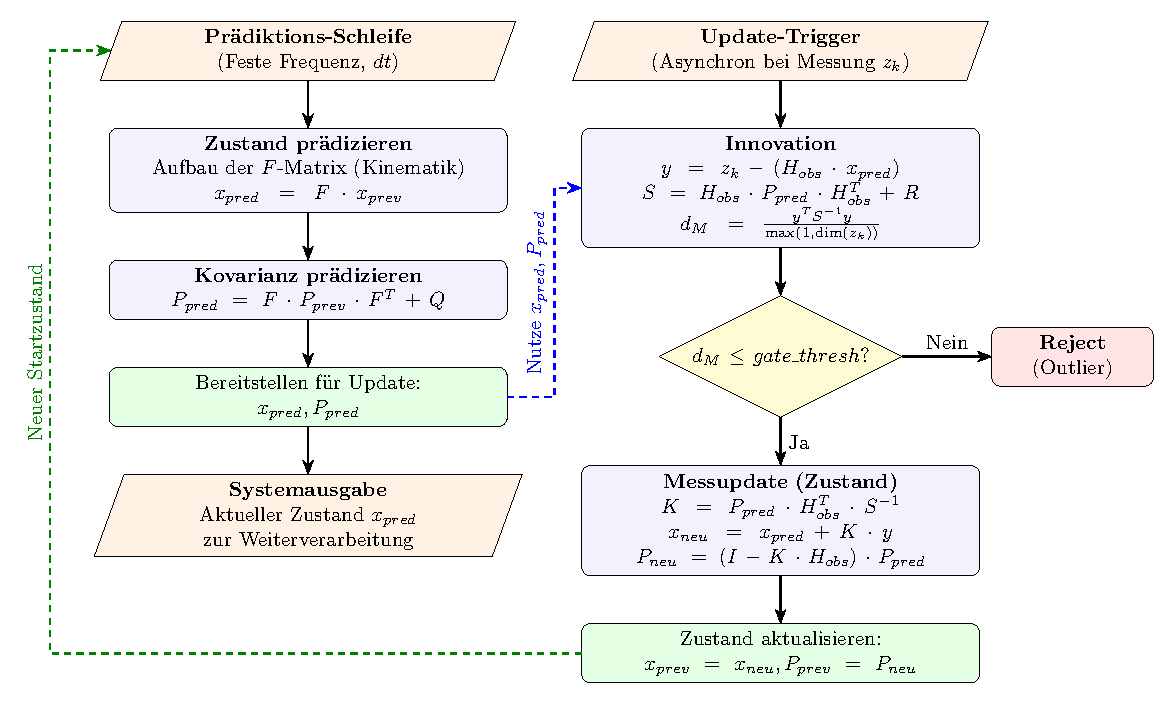
\includegraphics[width=\linewidth, height=0.6\textheight, keepaspectratio]{Figures/tikz/kf/kf.pdf}
    \caption{Ablaufdiagramm des KF.}
    \label{fig:kf_ablauf}
\end{figure}

\newpage
\subsection{Extended Kalman-Filter (EKF)}
\label{subsec:ekf}
\begin{figure}[htbp]
    \centering
    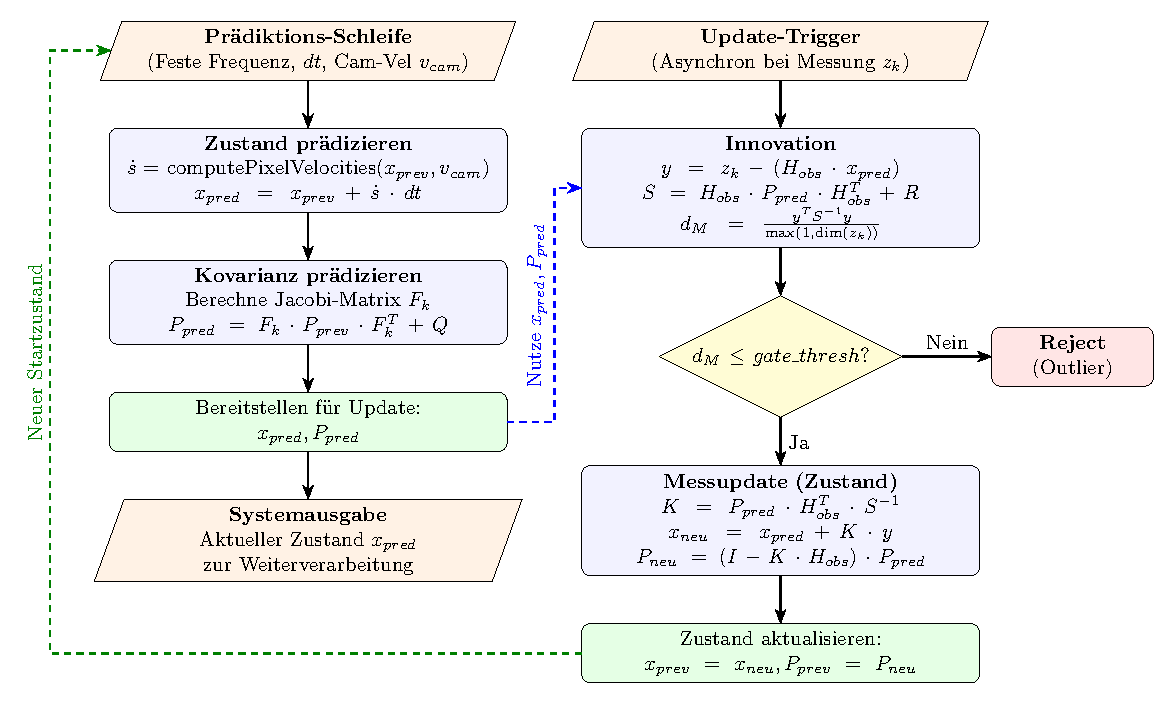
\includegraphics[width=\linewidth, height=0.6\textheight, keepaspectratio]{Figures/tikz/ekf/ekf.pdf}
    \caption{Ablaufdiagramm des EKF.}
    \label{fig:ekf_ablauf}
\end{figure}

\newpage
\subsection{Unscented Kalman-Filter (UKF)}
\label{subsec:ukf}
\begin{figure}[htbp]
    \centering
    \missingfigure[figwidth=\linewidth, figheight=0.6\textheight]{Figures/tikz/ukf/ukf.pdf}
    \caption{Ablaufdiagramm des UKF.}
    \label{fig:ukf_ablauf}
\end{figure}

\newpage
\subsection{Error State Kalman-Filter (ESKF)}
\label{subsec:eskf}
\begin{figure}[htbp]
    \centering
    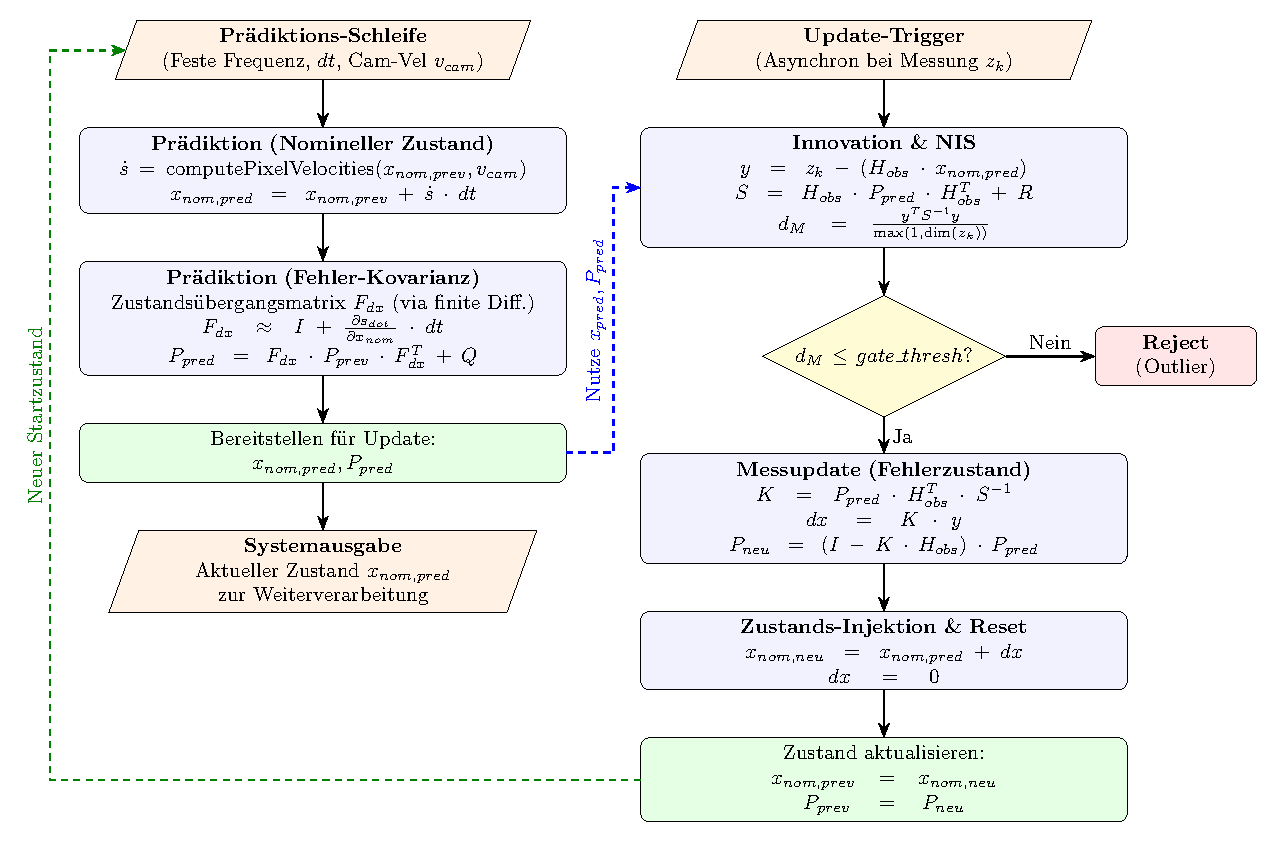
\includegraphics[width=\linewidth, height=0.6\textheight, keepaspectratio]{Figures/tikz/eskf/eskf.pdf}
    \caption{Ablaufdiagramm des ESKF.}
    \label{fig:ekf_ablauf}
\end{figure}

\newpage
\subsection{1\euro{}-Filter}
\label{subsec:1euro_filter}
\begin{figure}[htbp]
    \centering
    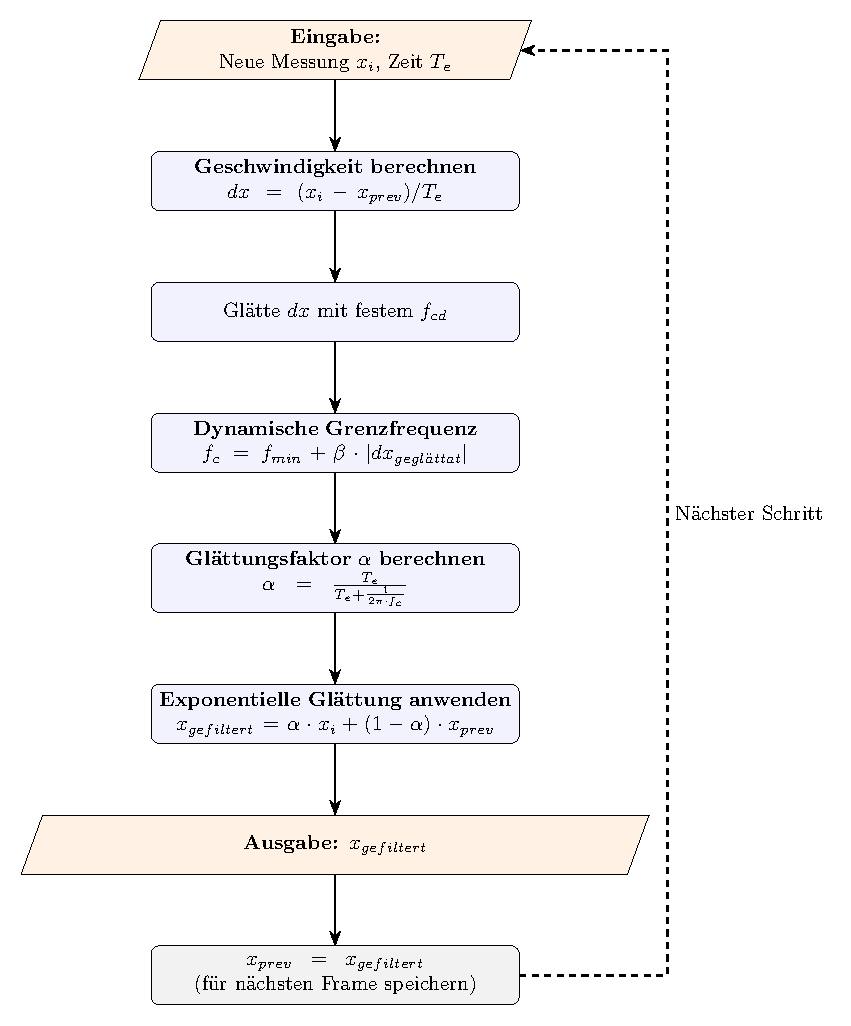
\includegraphics[width=\linewidth, height=0.6\textheight, keepaspectratio]{Figures/tikz/1euro_filter/1euro_filter.pdf}
    \caption{Ablaufdiagramm des 1\euro{}-Filters.}
    \label{fig:1euro_filter_ablauf}
\end{figure}
